%%%%%%%%%%%%%%%%%%%%%%%%%%%%%%%%%%%%%%%%%%%%%%%%%%%%%%%%%%%%%%%%%%%%%%
% Problem statement
\begin{statement}[
  problempoints=110,
  timelimit=1 second,
  memorylimit=512 MiB,
]{Zoo}

\setlength\intextsep{-0.1cm}
\begin{wrapfigure}[12]{r}{0.23\textwidth}
\centering

\includegraphics[width=0.23\textwidth]{img/tragovi.png}
\end{wrapfigure}

%\section

On a cold Christmas night in 2010, Zagreb was covered in snow.
Zdravko decided to leave his castle, cross the road and take a stroll through
the Maksimir park. Unfortunately, the idyllic winter evening was interrupted by
a monster that was lurking in the nearby bushes. The monster jumped in front of
Zdravko, but Zdravko roared a mighty roar which scared the monster away.
Unbeknownst to him, a bunch of animals from the nearby zoo were startled by
that roar. More precisely, a group of tigers and bulls were so annoyed that they
decided to escape the zoo in order to find a nice quiet place to sleep.

During their escape, the animals had to pass through a rectangular area divided
in $R \times C$ unit squares. The animals must enter the area through the
upper-left corner and must leave the area through the lower-right corner. In
order to escape as quietly as possible, animals will pass through this area
one by one, walking along an arbitrary path in four general directions (up,
down, left and right). In other words, each animal does
not necessarily travel along a shortest path during its escape
and it might step on the same unit square more than once (including the entrance
and exit). Since the ground is covered in snow, animals leave footprints when
they step inside unit squares. If another footprint is already in the square
that is about to be stepped on, the animal will erase the previous footprint and
leave a new one.

Your task is to determine the minimal number of animals that have
escaped the Maksimir zoo based on the footprints that were left in the
aforementioned rectangular area.

%%%%%%%%%%%%%%%%%%%%%%%%%%%%%%%%%%%%%%%%%%%%%%%%%%%%%%%%%%%%%%%%%%%%%%
% Input
\subsection*{Input}
The first line contains two integers $R$ and $C$ from the task description. \\
The next $R$ lines contain $C$ characters that represent the rectangular area
from the task description. Character \texttt{T} represents a tiger's footprint,
character \texttt{B} represents a bull's footprint and character \texttt{*}
represents untouched snow.

You can assume that the input data is such that at least one animal entered the
rectangular area and that each animal that entered the area has also left the
area according to the rules from the task description.

%%%%%%%%%%%%%%%%%%%%%%%%%%%%%%%%%%%%%%%%%%%%%%%%%%%%%%%%%%%%%%%%%%%%%%
% Output
\subsection*{Output}
Output the minimal number of animals that have escaped the zoo.

%%%%%%%%%%%%%%%%%%%%%%%%%%%%%%%%%%%%%%%%%%%%%%%%%%%%%%%%%%%%%%%%%%%%%%
% Scoring
\subsection*{Scoring}
{\renewcommand{\arraystretch}{1.4}
  \setlength{\tabcolsep}{6pt}
  \begin{tabular}{ccl}
 Subtask & Score & Constraints \\ \midrule
  1 & 45 & $2 \le R, C \le 100$ \\
  2 & 65 & $2 \le R, C \le 1000$ \\
\end{tabular}}

%%%%%%%%%%%%%%%%%%%%%%%%%%%%%%%%%%%%%%%%%%%%%%%%%%%%%%%%%%%%%%%%%%%%%%
% Examples
\subsection*{Examples}
\begin{tabularx}{\textwidth}{X'X'X}
\sampleinputs{test/zoo.dummy.in.1}{test/zoo.dummy.out.1} &
\sampleinputs{test/zoo.dummy.in.2}{test/zoo.dummy.out.2} &
\sampleinputs{test/zoo.dummy.in.3}{test/zoo.dummy.out.3}
\end{tabularx}

\textbf{Clarification of the second example:}

\begin{wrapfigure}{c}{\textwidth}
\centering
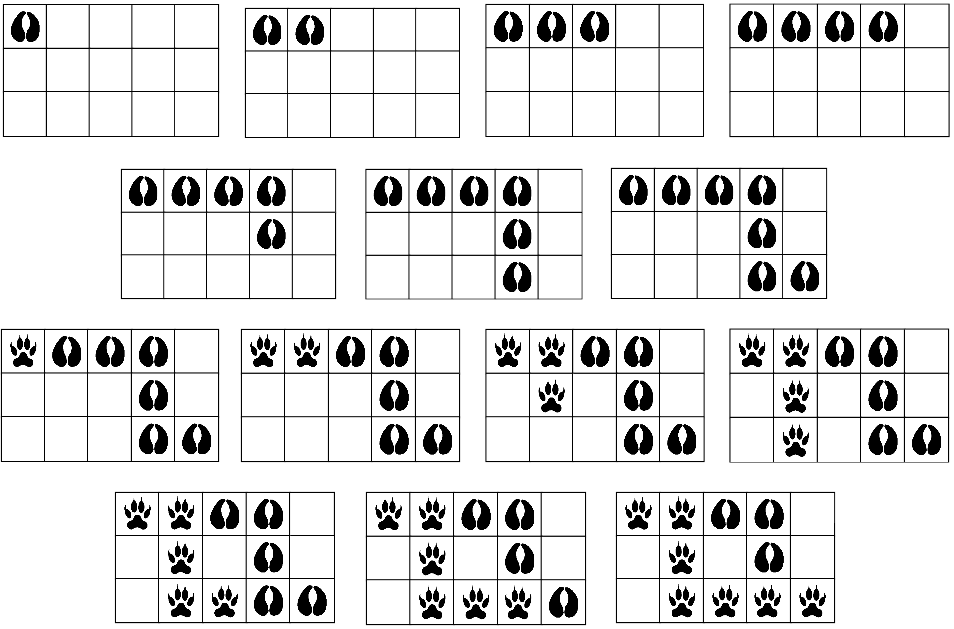
\includegraphics[width=\textwidth]{img/escape.png}
\end{wrapfigure}

%%%%%%%%%%%%%%%%%%%%%%%%%%%%%%%%%%%%%%%%%%%%%%%%%%%%%%%%%%%%%%%%%%%%%%
% We're done
\end{statement}

%%% Local Variables:
%%% mode: latex
%%% mode: flyspell
%%% ispell-local-dictionary: "croatian"
%%% TeX-master: "../hio.tex"
%%% End:
